\documentclass[11pt]{article}

\usepackage[letterpaper,margin=0.78in,headheight=15pt]{geometry}
\usepackage[T1]{fontenc}
\usepackage[utf8]{inputenc}
\usepackage{lmodern}
\usepackage{microtype}
\usepackage{graphicx}
\usepackage{booktabs}
\usepackage{siunitx}
\usepackage{xcolor}
\usepackage{hyperref}
\usepackage{fancyhdr}
\usepackage{titlesec}
\usepackage{caption}
\usepackage{enumitem}
\usepackage{float}

\definecolor{navy}{HTML}{17365D}
\definecolor{blue}{HTML}{2E75B6}
\definecolor{lightblue}{HTML}{D9EAF7}
\definecolor{orange}{HTML}{D55E00}
\definecolor{graytext}{HTML}{555555}

\hypersetup{
  colorlinks=true,
  linkcolor=navy,
  urlcolor=blue,
  pdftitle={Heating-Plant Vibration Evidence and Laboratory Comparison},
  pdfsubject={Concise peak-centered assessment of building vibration measurements}
}
\graphicspath{{../figures/}}
\sisetup{detect-all,round-mode=figures,round-precision=3}
\DeclareSIUnit{\sqrthertz}{\hertz\tothe{0.5}}
\newcommand{\asdunit}{\si{\meter\per\second\squared\per\sqrthertz}}
\newcommand{\freq}[1]{\SI[scientific-notation=false]{#1}{\hertz}}

\pagestyle{fancy}
\fancyhf{}
\lhead{\textcolor{graytext}{Heating-Plant Vibration Evidence}}
\rhead{\textcolor{graytext}{Physics Laboratories}}
\cfoot{\thepage}
\renewcommand{\headrulewidth}{0.4pt}

\titleformat{\section}{\Large\bfseries\color{navy}}{\thesection}{0.7em}{}
\captionsetup{font=small,labelfont=bf}
\setlist{nosep,leftmargin=1.5em}
\setlength{\parindent}{0pt}
\setlength{\parskip}{0.50em}
\renewcommand{\arraystretch}{1.14}

\begin{document}
	
	\begin{titlepage}
		\centering
		\vspace*{1.2in}
		{\color{navy}\rule{\textwidth}{1.2pt}\par}
		\vspace{0.45in}
		{\Huge\bfseries Building Vibration Measurement Analysis\par}
		\vspace{0.18in}
		{\Large Laboratory ranking, source signatures, and optical-table performance\par}
		\vspace{0.45in}
		{\color{navy}\rule{\textwidth}{1.2pt}\par}
		\vfill
		\begin{tabular}{rl}
			\textbf{Source workbook:} & \texttt{FinalReportData.xlsx}\\
			\textbf{Measurements:} & 15 spectra in 5 measured rooms\\
			\textbf{Spectral range:} & 0--250.25 Hz at 0.48877 Hz resolution\\
			\textbf{Report date:} & July 23, 2026\\
		\end{tabular}
		\vfill
		{\large Prepared as a data-driven assessment for vibration-sensitive experimental work\par}
	\end{titlepage}

\section{Evidence for the heating plant}

\begin{figure}[H]
\centering
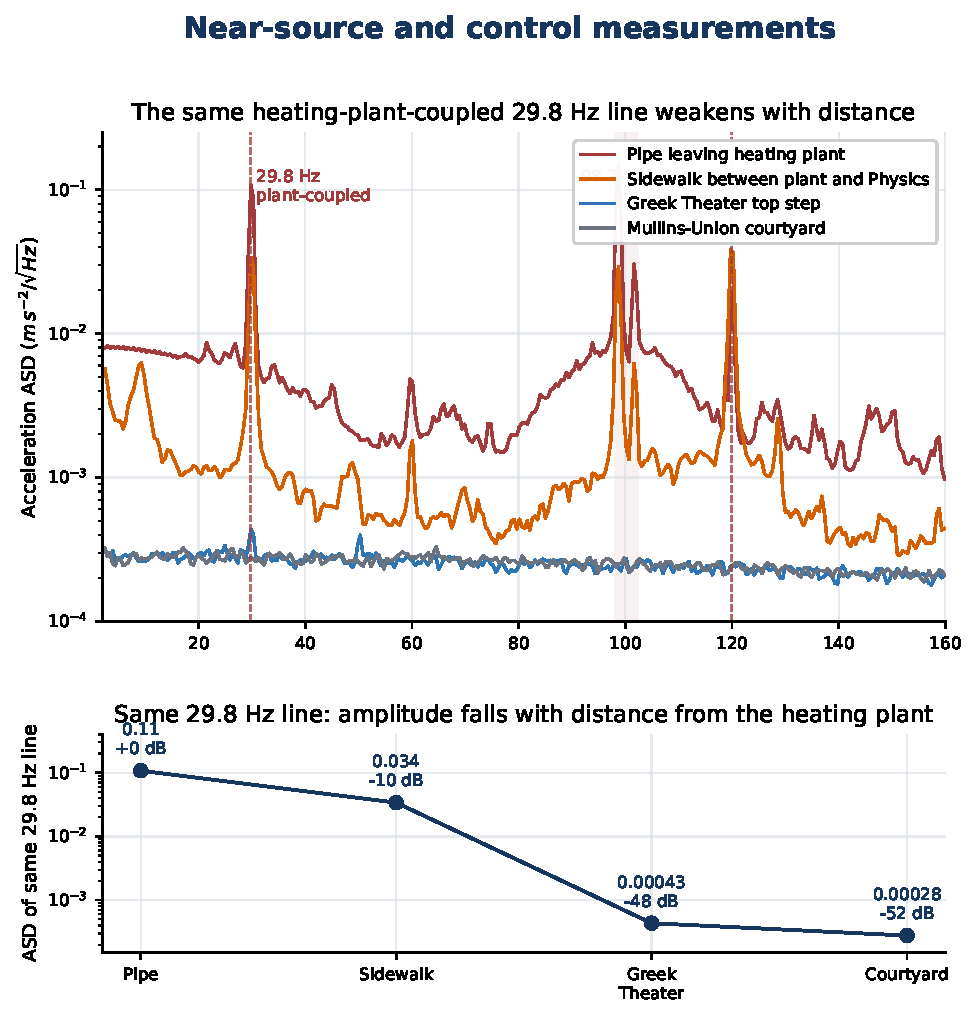
\includegraphics[width=\linewidth]{source_distance_evidence.pdf}
\caption{The same heating-plant-coupled \freq{29.8} line falls from
\SI{0.108}{\meter\per\second\squared\per\sqrthertz} on the plant pipe to
\SI{0.0339}{\meter\per\second\squared\per\sqrthertz} on the sidewalk, then
approaches the remote background. The same near-to-far pattern is visible at
other plant-associated frequencies.}
\end{figure}

The common frequency and its approximately \SI{52}{\decibel} drop from the
pipe to the courtyard identify the \freq{29.8} peak seen inside Physics as
\textbf{the same vibration coupled from the heating plant}, not separate
room-generated peaks or a sensor resonance.

\newpage
\section{Heating-plant spectral fingerprint}

\begin{table}[H]
\centering
\caption{Acceleration ASD at recurring plant-associated frequencies.
All entries are in $10^{-3}$ \asdunit. Values are read at the common
frequency bin nearest each listed line.}
\resizebox{\textwidth}{!}{%
\begin{tabular}{lrrrrrrr}
\toprule
Frequency & Plant pipe & Sidewalk & Herzog & PHYS 111 & Titan & PHYS 245 & PHYS 244\\
\midrule
29.8 Hz  & 107.68 & 33.90 & 22.87 & 17.97 & 5.15 & 2.19 & 1.41\\
98.7 Hz  & 148.13 & 29.14 & 3.09  & 1.65  & 0.26 & 0.28 & 0.23\\
101.7 Hz & 30.43  & 6.21  & 0.74  & 0.46  & 0.21 & 0.29 & 0.32\\
120.0 Hz & 18.86  & 38.58 & 2.41  & 0.59  & 0.23 & 0.26 & 0.58\\
\bottomrule
\end{tabular}}
\end{table}

The \freq{29.8} row tracks the same heating-plant-coupled vibration from the
plant pipe into the Physics rooms. Its matching frequency and spatial decay
are the principal source evidence. The group near
\SIrange{98.7}{101.7}{\hertz} and the \freq{120.0} line provide additional
corroboration. Exact amplitudes need not scale monotonically at every
frequency because propagation, local structural resonances, and operating
conditions differ among measurements.

\begin{figure}[H]
\centering
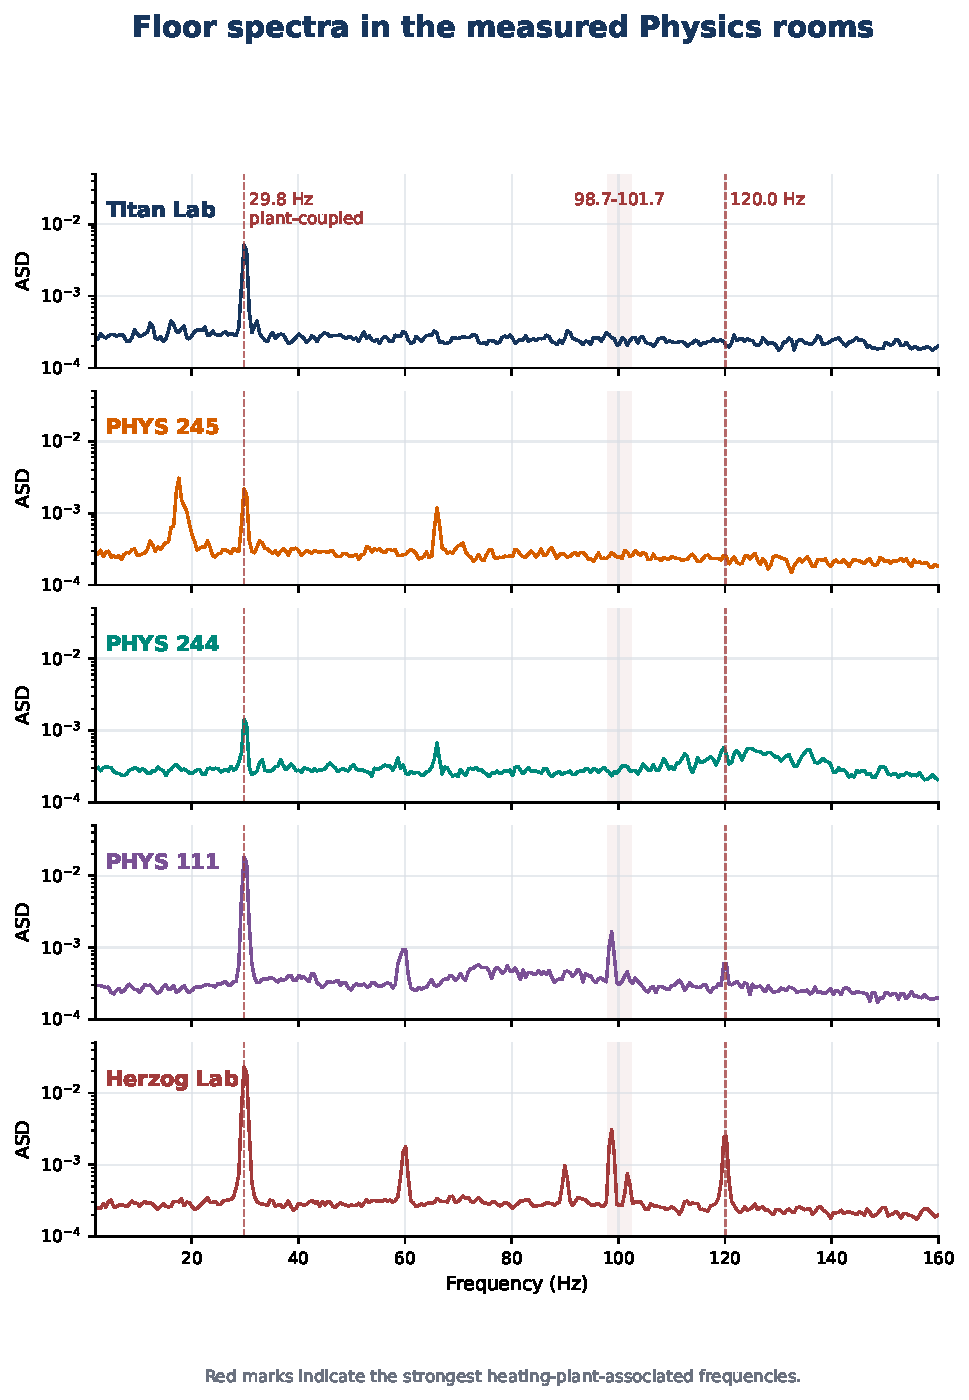
\includegraphics[height=0.80\textheight,keepaspectratio]{all_floor_spectra.pdf}
\caption{Floor spectra for the five measured Physics rooms, kept on common
axes. The red marker at \freq{29.8} follows the same vibration coupled from
the heating plant; the other red markers identify additional
plant-associated frequencies.}
\end{figure}

\newpage
\section{Room choice}

\begin{figure}[H]
\centering
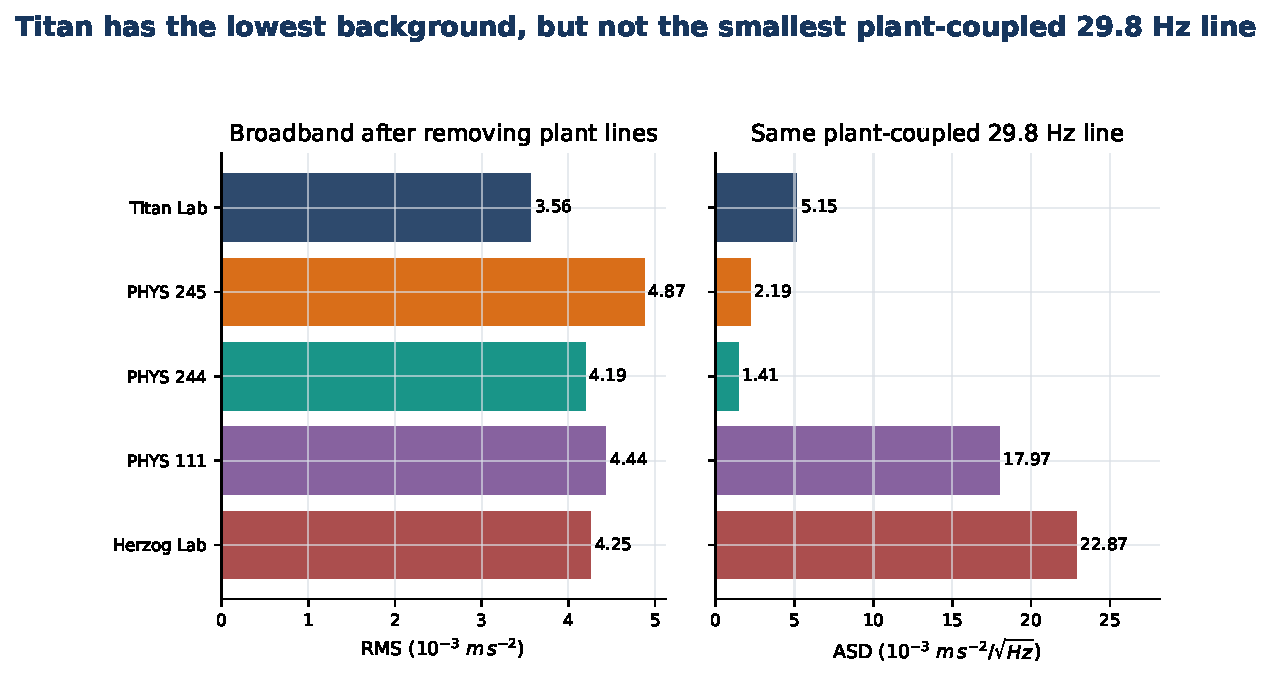
\includegraphics[width=0.97\linewidth]{room_choice_context.pdf}
\caption{Two complementary room metrics. The left panel removes narrow
plant-associated lines to compare broadband background.
The right panel compares the amplitude of the same heating-plant-coupled
\freq{29.8} line in each room.}
\end{figure}

The left panel explains why Titan appears so quiet in the spectra: after the
coherent plant lines are set aside, it has the lowest band-integrated
background of the five rooms. The right panel prevents that result from being
overstated. PHYS 244 and PHYS 245 receive the same \freq{29.8} vibration at
smaller amplitude, while its amplitude is substantially larger in Herzog and
PHYS 111.

\fcolorbox{orange}{white}{%
  \begin{minipage}{0.93\linewidth}
  \textbf{\color{navy}Where I would build an optics laboratory:}
  I would consider Titan.  It does have a significantly stronger 30Htz line from the plant, and that needs to be considered as that low frequency likes to go right through floated legs, but a floated table will help dampen it out somewhat and I suspect an ACTIVELY damped table will have little issues making it all but disappear--albeit at some expense.  The rest of the spectrum is exceedingly low in the Titan lab so it was very well isolated for that TEM that was there some time ago.  PHYS 245 would
  be my next choice and could be preferable for apparatus mechanically
  sensitive to this same \freq{29.8} vibration or if active dampening is not an option at which point you basically want as far away from the heating plant as possible and 245 gets you there.
  \end{minipage}
}

\newpage
\section{What the optical tables accomplish}

\begin{figure}[H]
\centering
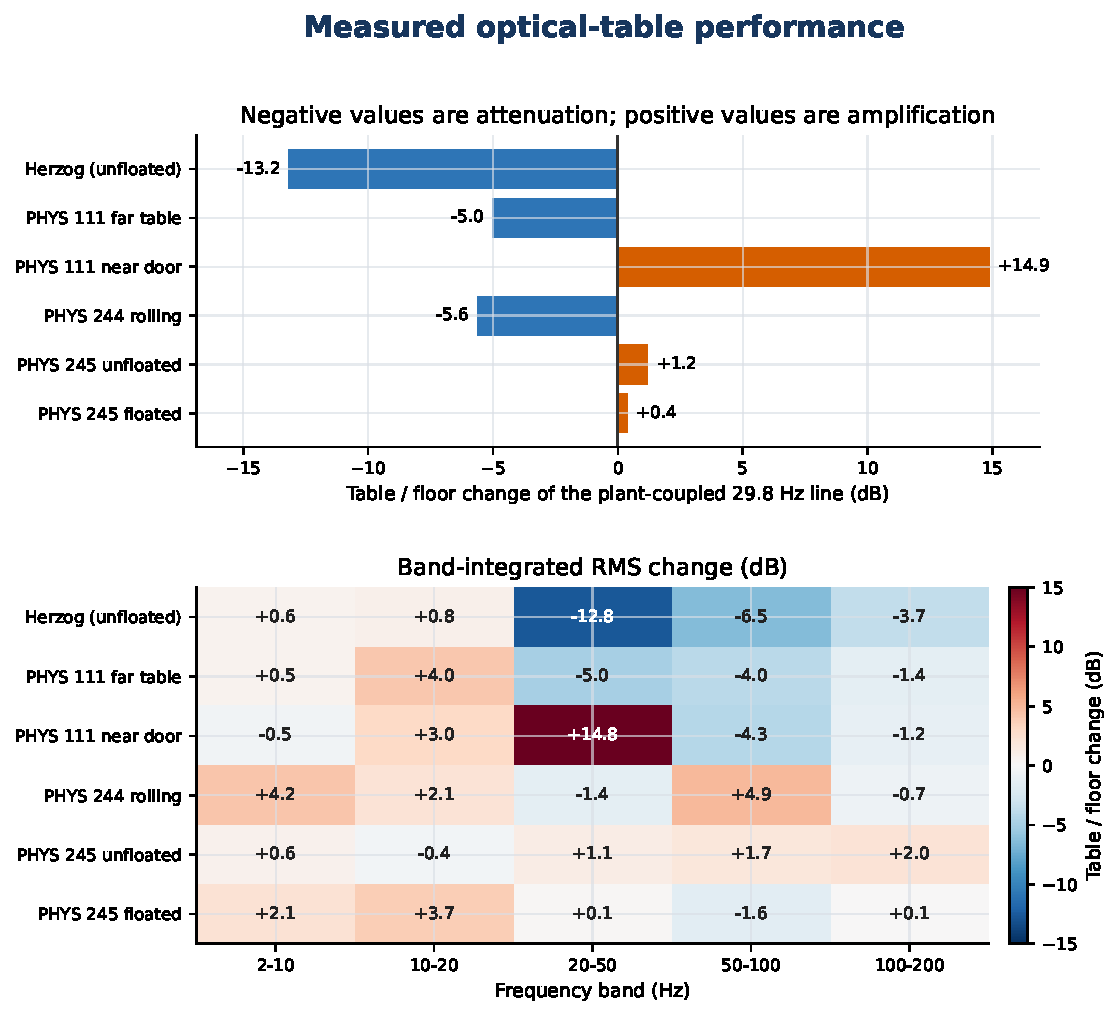
\includegraphics[width=0.96\linewidth]{optical_table_performance.pdf}
\caption{Measured table-to-floor change. Negative values mean attenuation;
positive values mean amplification. The upper panel isolates the same
heating-plant-coupled \freq{29.8} line; the lower panel summarizes broader
bands.}
\end{figure}

The plot shows the measured change from each room floor to its table. Herzog
has the largest reduction of the heating-plant-coupled \freq{29.8} line, which
is not surprising because this line is much larger on the Herzog floor to
begin with. Its remaining table amplitude is about
\SI{0.0050}{\meter\per\second\squared\per\sqrthertz}: lower than the PHYS 111
table measurements, but about twice the PHYS 245 table level and roughly
seven times the PHYS 244 rolling-table level at this frequency.

\newpage
\section{Herzog: reduced, but still exposed}

\begin{figure}[H]
\centering
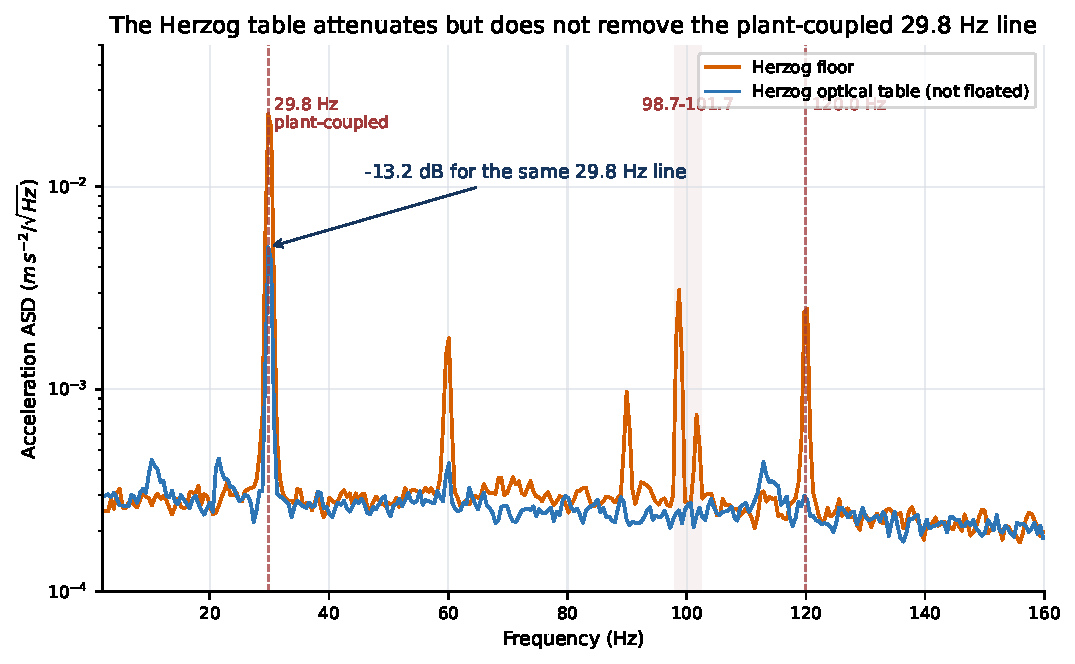
\includegraphics[width=\linewidth]{herzog_floor_vs_table.pdf}
\caption{Herzog floor and optical-table spectra only. The freezer-top and
back-counter traces are intentionally omitted.}
\end{figure}

The plot shows that the unfloated Herzog table reduces the same
heating-plant-coupled \freq{29.8} floor line by \SI{13.2}{\decibel}, but
leaves a clear residual amplitude of approximately
\SI{0.0050}{\meter\per\second\squared\per\sqrthertz}.

\section*{Concise conclusion}

The spatial controls, the plant-pipe measurement, and the recurring spectral
fingerprint together make the heating plant the almost-certain source region
for the low-frequency vibration observed in Herzog. The turbine is the most
plausible individual source given the timing of the problem, but a short
generator-free measurement tied to turbine operating state would provide the
cleanest final confirmation. For room selection, Titan has the best broadband
background; PHYS 245 receives the same heating-plant-coupled \freq{29.8}
vibration at smaller amplitude and is the principal alternative as that
frequency is especially difficult for an optical table to isolate.  Obviously there is way in Hades I would put an optics lab in the Herzog lab.  The very unfortunate thing for the entire building is that 29.8Hz is evidently difficult to filter even with a floated table.  

\end{document}
